\chapter*{Acknowledgements}
\addcontentsline{toc}{chapter}{Acknowledgements}

\section*{Institutions}

We thank Columbia University along with the Departments of
Statistics and Political Science, the Applied Statistics Center, the
Institute for Social and Economic Research and Policy ({\sc iserp}),
and the Core Research Computing Facility.

\section*{Grants}

\Stan was supported in part by 
%
the U.~S.\ Department of Energy 
({\small DE-SC0002099}), 
%
the U.~S.\ National Science Foundation 
{\small ATM-0934516}
``Reconstructing Climate from Tree Ring Data.''
and 
%
the U.~S.\ Department of Education Institute of Education Sciences 
({\small ED-GRANTS-032309-005}:
 ``Practical Tools for Multilevel Hierarchical Modeling in Education
 Research'' and
 {\small R305D090006-09A}:
 ``Practical solutions for missing data'').
%
The high-performance computing
facility on which we ran evaluations was made possible through 
a grant from the U.~S.\ National Institutes of Health 
({\small 1G20RR030893-01}:
 ``Research Facility Improvement Grant'').

\Stan is currently supported in part by a grant from the National
Science Foundation (CNS-1205516)

\section*{Individuals}

We thank Michael Betancourt for hanging out at our meetings and
sharing his insights into differential geometry, John Salvatier for
pointing us to automatic differentiation and \HMC in the first place,
and Kristen van Leuven of {\sc iserp} for help preparing our grant
proposals.

\vfill
\begin{center}
\hfill
\begin{minipage}[b]{2in}
  \footnotesize {\it Stanislaw Ulam, namesake of \Stan and co-inventor
    of Monte Carlo methods \citep{MetropolisUlam:1949}, shown here
    holding the Fermiac, Enrico Fermi's physical Monte Carlo simulator
    for neutron diffusion.}
  \\[3pt] \mbox{ } \hfill
  {\scriptsize Image from \citep{Giesler:2000}.}
\end{minipage} \ \ \ \ \ 
\begin{minipage}[b]{1.5in} \mbox{ } \hfill
  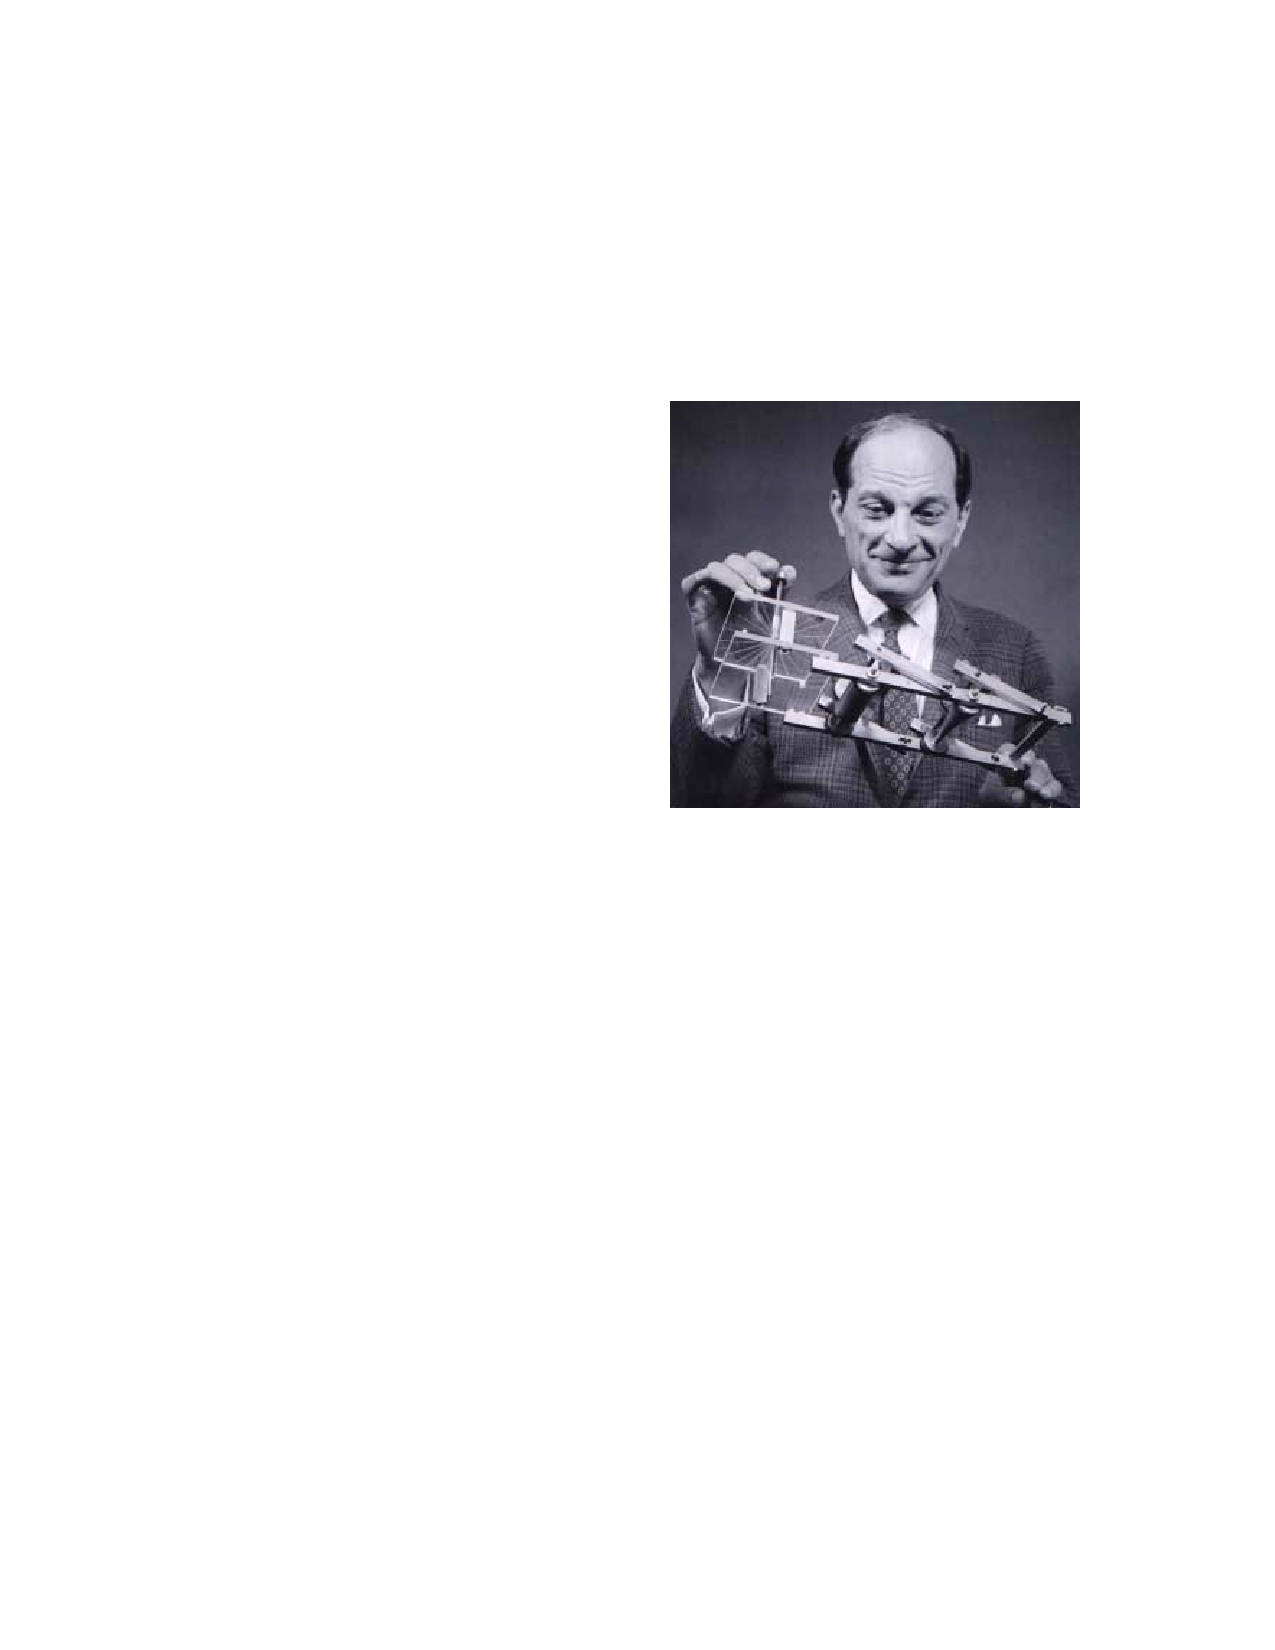
\includegraphics[width=1.5in]{../../../logos/ulam-fermiac.pdf}
\end{minipage} 
\end{center}
